```latex
\section{UI-Mockups}
\label{sec:ui-mockups}

Die Mockups dienen zur Veranschaulichung des geplanten Bedienkonzepts. Weitere Zustände und Randfälle sind im
interaktiven Figma-Prototyp umgesetzt.

Der interaktive Prototyp kann in Figma ausprobiert werden:
\href{https://www.figma.com/proto/x5hqdUGYxCmE8HOd1pPbDU/SkinSentry?node-id=4-8963&p=f&t=uXjVH2q8rO4hvudf-1&scaling=min-zoom&content-scaling=fixed&page-id=0%3A1&starting-point-node-id=4%3A8684&show-proto-sidebar=1}
{SkinSentry -- interaktiver Figma-Prototyp}

\subsection{Übersicht und Navigation}

\begin{figure}[htbp]
    \centering
    \begin{minipage}[t]{0.48\textwidth}
        \centering
        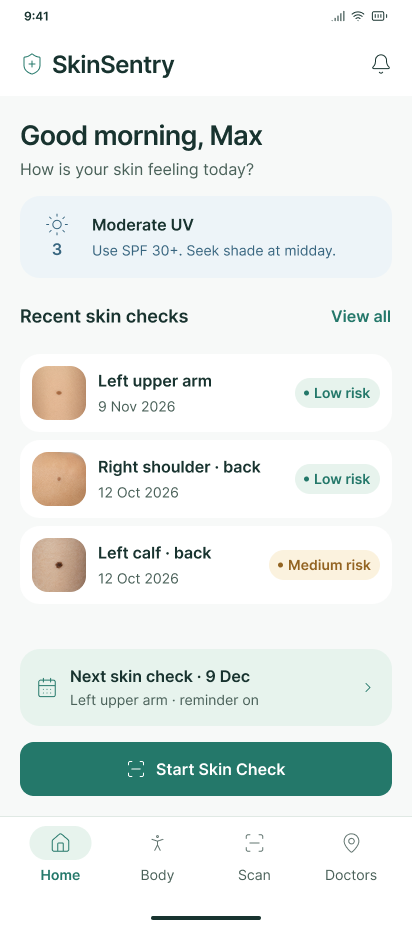
\includegraphics[width=0.82\linewidth]{images/ui-mock/01_home.png}

        \small (a) Startseite
    \end{minipage}
    \hfill
    \begin{minipage}[t]{0.48\textwidth}
        \centering
        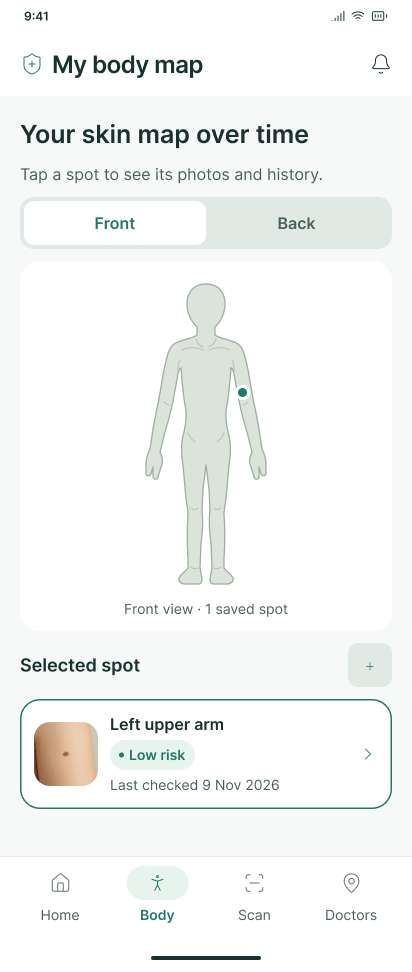
\includegraphics[width=0.82\linewidth]{images/ui-mock/02_body_map_front.png}

        \small (b) 2D-Körperübersicht
    \end{minipage}
    \caption{Startseite und Körperübersicht von SkinSentry}
    \label{fig:ui-overview}
\end{figure}

\begin{figure}[htbp]
    \centering
    \includegraphics[width=0.42\textwidth]{images/ui-mock/03_spot_history.png}
    \caption{Verlauf einer gespeicherten Hautstelle}
    \label{fig:spot-history}
\end{figure}

\clearpage

\subsection{Ablauf des Skin Checks}

\begin{figure}[htbp]
    \centering
    \begin{minipage}[t]{0.48\textwidth}
        \centering
        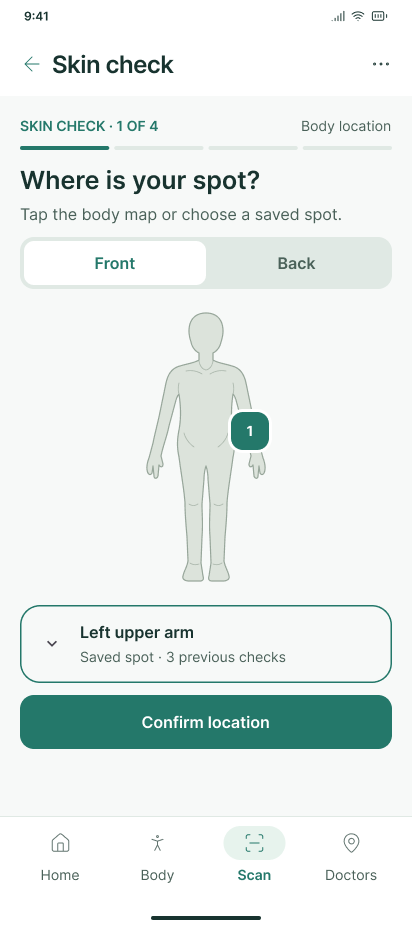
\includegraphics[width=0.82\linewidth]{images/ui-mock/04_body_location.png}

        \small (a) Auswahl der Körperstelle
    \end{minipage}
    \hfill
    \begin{minipage}[t]{0.48\textwidth}
        \centering
        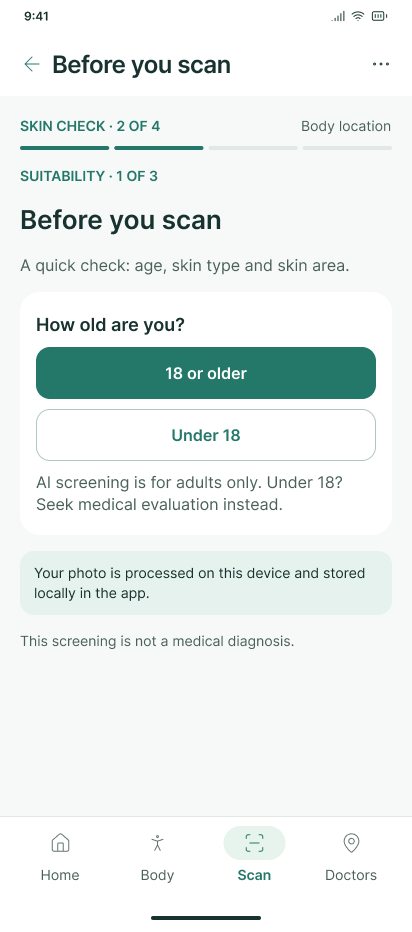
\includegraphics[width=0.82\linewidth]{images/ui-mock/05_suitability_age.png}

        \small (b) Altersprüfung
    \end{minipage}
    \caption{Beginn des Skin-Check-Ablaufs}
    \label{fig:scan-start}
\end{figure}

\begin{figure}[htbp]
    \centering
    \begin{minipage}[t]{0.48\textwidth}
        \centering
        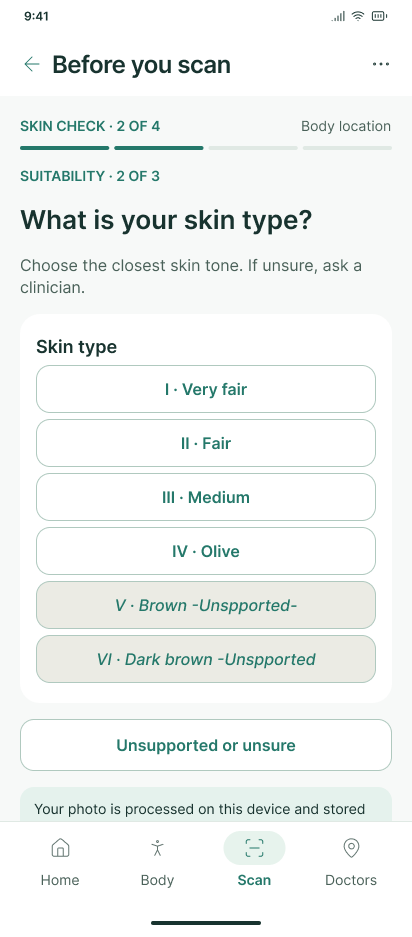
\includegraphics[width=0.82\linewidth]{images/ui-mock/06_suitability_skin_type.png}

        \small (a) Auswahl des Hauttyps
    \end{minipage}
    \hfill
    \begin{minipage}[t]{0.48\textwidth}
        \centering
        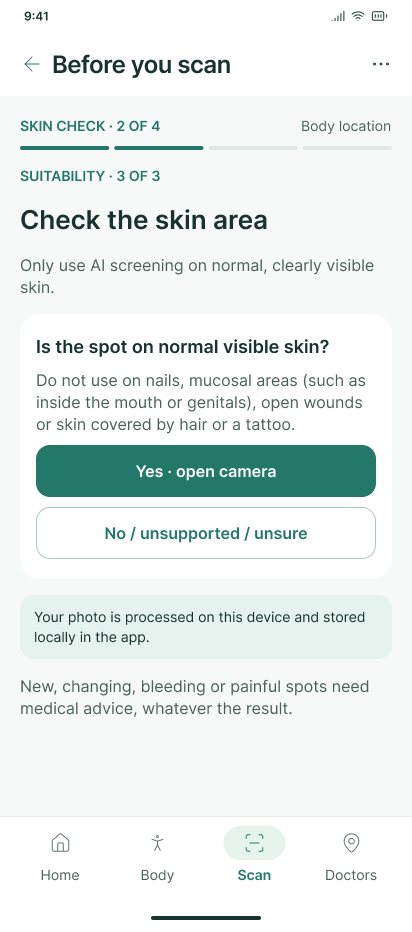
\includegraphics[width=0.82\linewidth]{images/ui-mock/07_suitability_skin_area.png}

        \small (b) Prüfung der Hautstelle
    \end{minipage}
    \caption{Eignungsprüfung vor dem Screening}
    \label{fig:suitability}
\end{figure}

\begin{figure}[htbp]
    \centering
    \begin{minipage}[t]{0.48\textwidth}
        \centering
        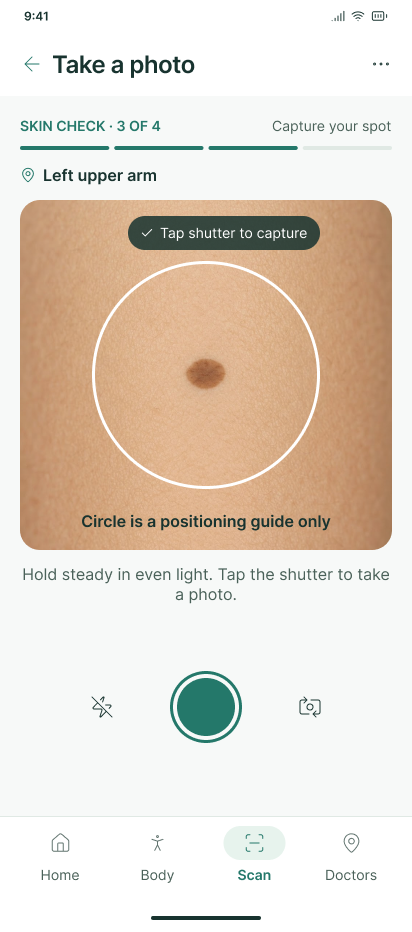
\includegraphics[width=0.82\linewidth]{images/ui-mock/08_camera.png}

        \small (a) Geführte Fotoaufnahme
    \end{minipage}
    \hfill
    \begin{minipage}[t]{0.48\textwidth}
        \centering
        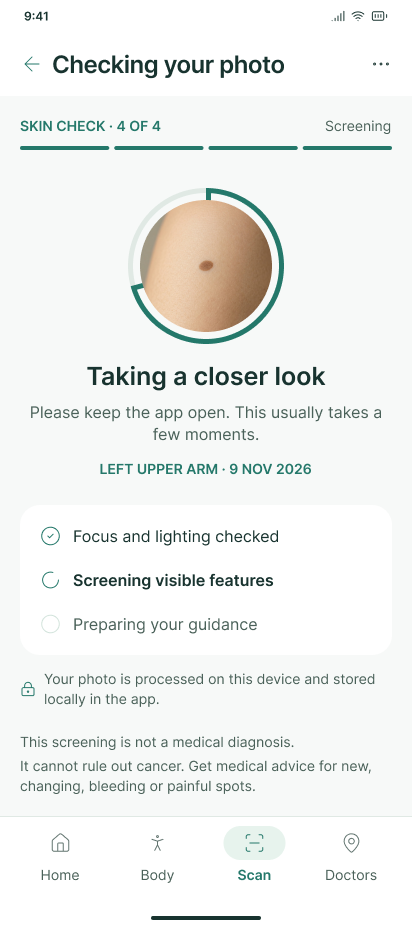
\includegraphics[width=0.82\linewidth]{images/ui-mock/09_screening.png}

        \small (b) Lokale Analyse
    \end{minipage}
    \caption{Fotoaufnahme und lokale Analyse}
    \label{fig:camera-screening}
\end{figure}

\clearpage

\subsection{Risikoeinschätzung und Handlungsempfehlung}

\begin{figure}[htbp]
    \centering
    \begin{minipage}[t]{0.48\textwidth}
        \centering
        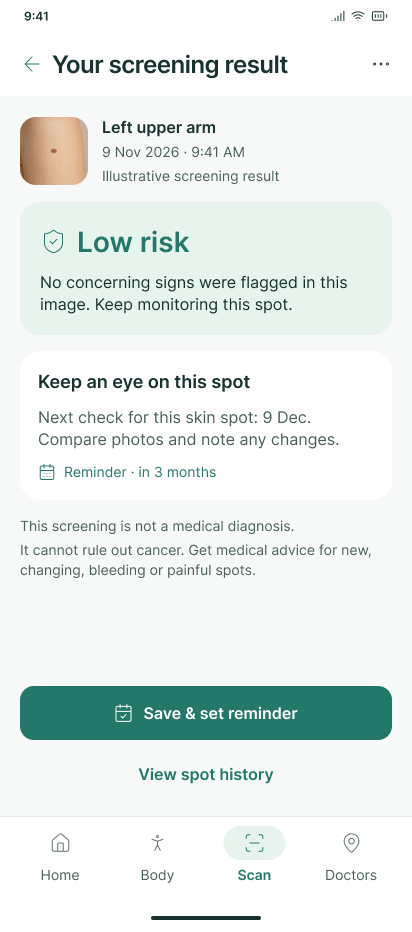
\includegraphics[width=0.82\linewidth]{images/ui-mock/10_result_low.png}

        \small (a) Niedriges Risiko
    \end{minipage}
    \hfill
    \begin{minipage}[t]{0.48\textwidth}
        \centering
        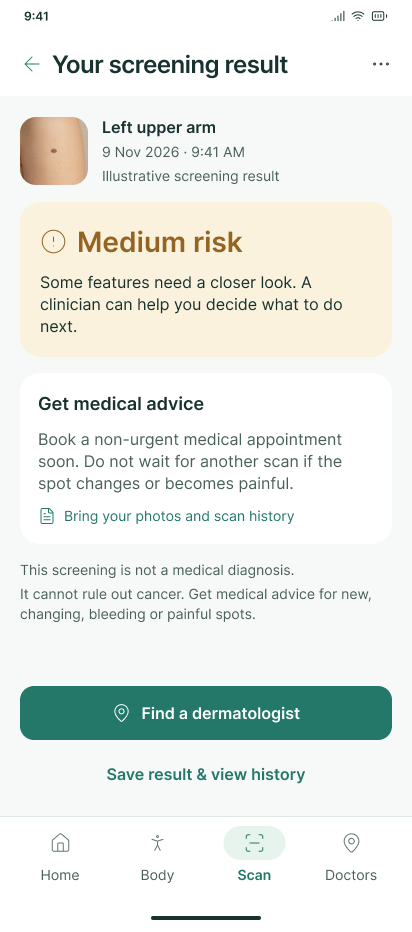
\includegraphics[width=0.82\linewidth]{images/ui-mock/11_result_medium.png}

        \small (b) Mittleres Risiko
    \end{minipage}
    \caption{Ergebnisansichten für niedriges und mittleres Risiko}
    \label{fig:risk-results-low-medium}
\end{figure}

\begin{figure}[htbp]
    \centering
    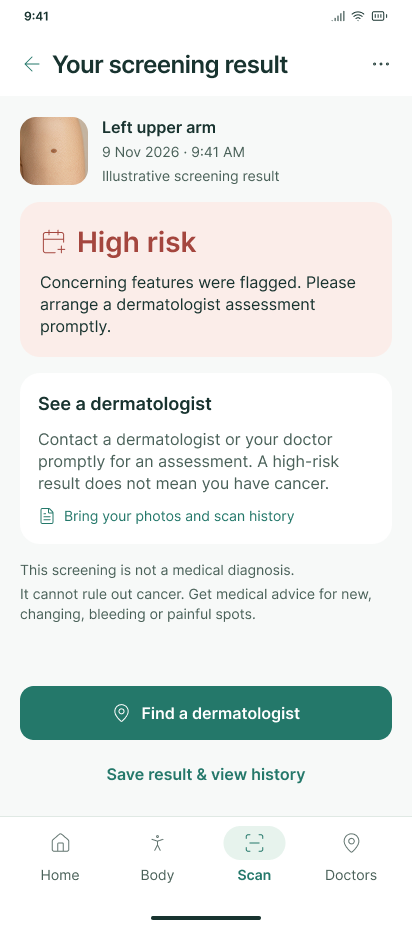
\includegraphics[width=0.42\textwidth]{images/ui-mock/12_result_high.png}
    \caption{Ergebnisansicht bei hohem Risiko}
    \label{fig:risk-result-high}
\end{figure}

\clearpage

\subsection{Weitere Zustände}

\begin{figure}[htbp]
    \centering
    \begin{minipage}[t]{0.48\textwidth}
        \centering
        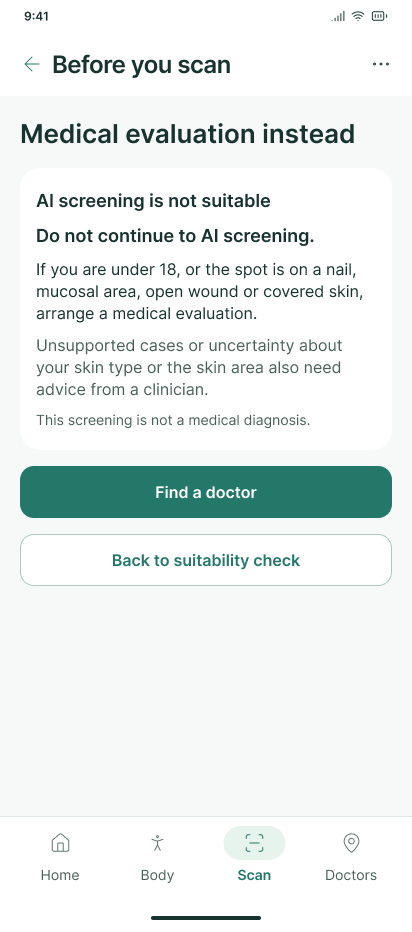
\includegraphics[width=0.82\linewidth]{images/ui-mock/13_medical_evaluation.png}

        \small (a) Verweis auf ärztliche Abklärung
    \end{minipage}
    \hfill
    \begin{minipage}[t]{0.48\textwidth}
        \centering
        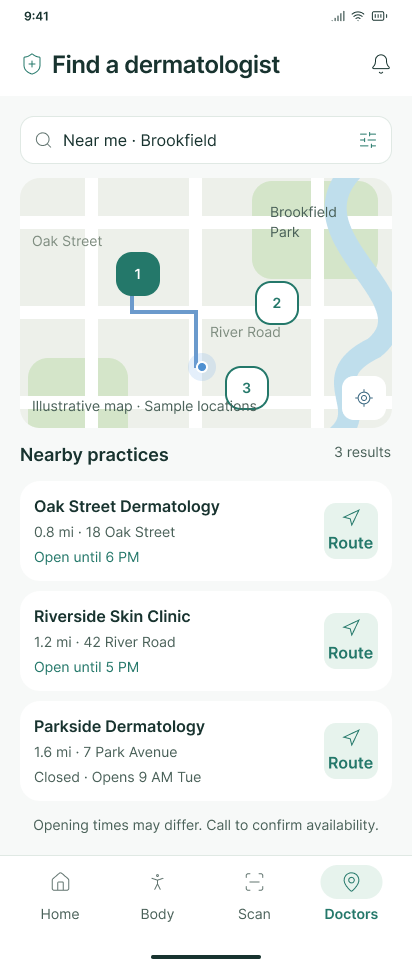
\includegraphics[width=0.82\linewidth]{images/ui-mock/14_doctors.png}

        \small (b) Optionale Arztsuche
    \end{minipage}
    \caption{Weitere im Mockup dargestellte Zustände}
    \label{fig:additional-states}
\end{figure}
```